\documentclass[12pt, letterpaper]{article}
\usepackage[utf8]{inputenc}
\usepackage{indentfirst}
\usepackage{graphicx}
\usepackage{setspace}
\usepackage[numbers]{natbib}
\usepackage [autostyle, english = american]{csquotes}
\MakeOuterQuote{"}
\usepackage{layout}
\usepackage[title]{appendix}
\usepackage[justification=centering]{caption}
\usepackage{titlesec}


\begin{document}

\setcounter{secnumdepth}{-1}
\titlespacing*{\section}{0pt}{2\baselineskip}{.33333\baselineskip}

%Cover page: 5pts
\title{MA348 Numerical Analysis, SUBJECT}
\author{David Jefts}
\date{\today}
\begin{titlepage}
	\centering
	\maketitle
	\centering
	\hfill
	\vfill
\end{titlepage}

\setlength{\voffset}{-0.5in}
\setlength{\headsep}{10pt}

%Introduction: 5pts
%Describe the problem and state objectives
\section{Introduction}
	Describe the problem and state objectives

%Theory-Analysis: 5pts
%State assumptions and develop equations
\section{Theory-Analysis}
State assumptions and develop equations

%Numerical Solution: 20pts
%Describe the numerical methods used to solve the problem
\section{Numerical Solution}
	Describe the numerical methods used to solve the problem

%Results and Discussion: 45pts
%Tabulate and plot the results, compare results, and discuss the accuracy of results
\section{Results and Discussion}
	Tabulate and plot the results, compare results, and discuss the accuracy of results
	
%Conclusions: 20pts
%Comment on the efficiency of the solvers
\section{Conclusions}
	Comment on the efficiency of the solvers

\pagebreak
	
%Appendices
%Include listings of the source codes, include printed copies of the output files
\appendix
	\section{Appendix A}
		\begin{figure}[h]
			\centering
			%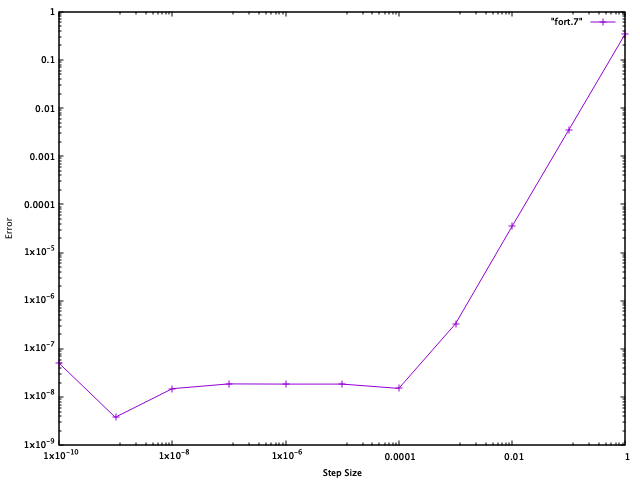
\includegraphics[width=\linewidth]{StepVsErrorGraph.png}
			%\caption{Graph of step-size vs error}
			%\label{fig:graph}
		\end{figure}
	\pagebreak
	
	\section{Appendix B}
		\begin{figure}[h]
			\centering
			%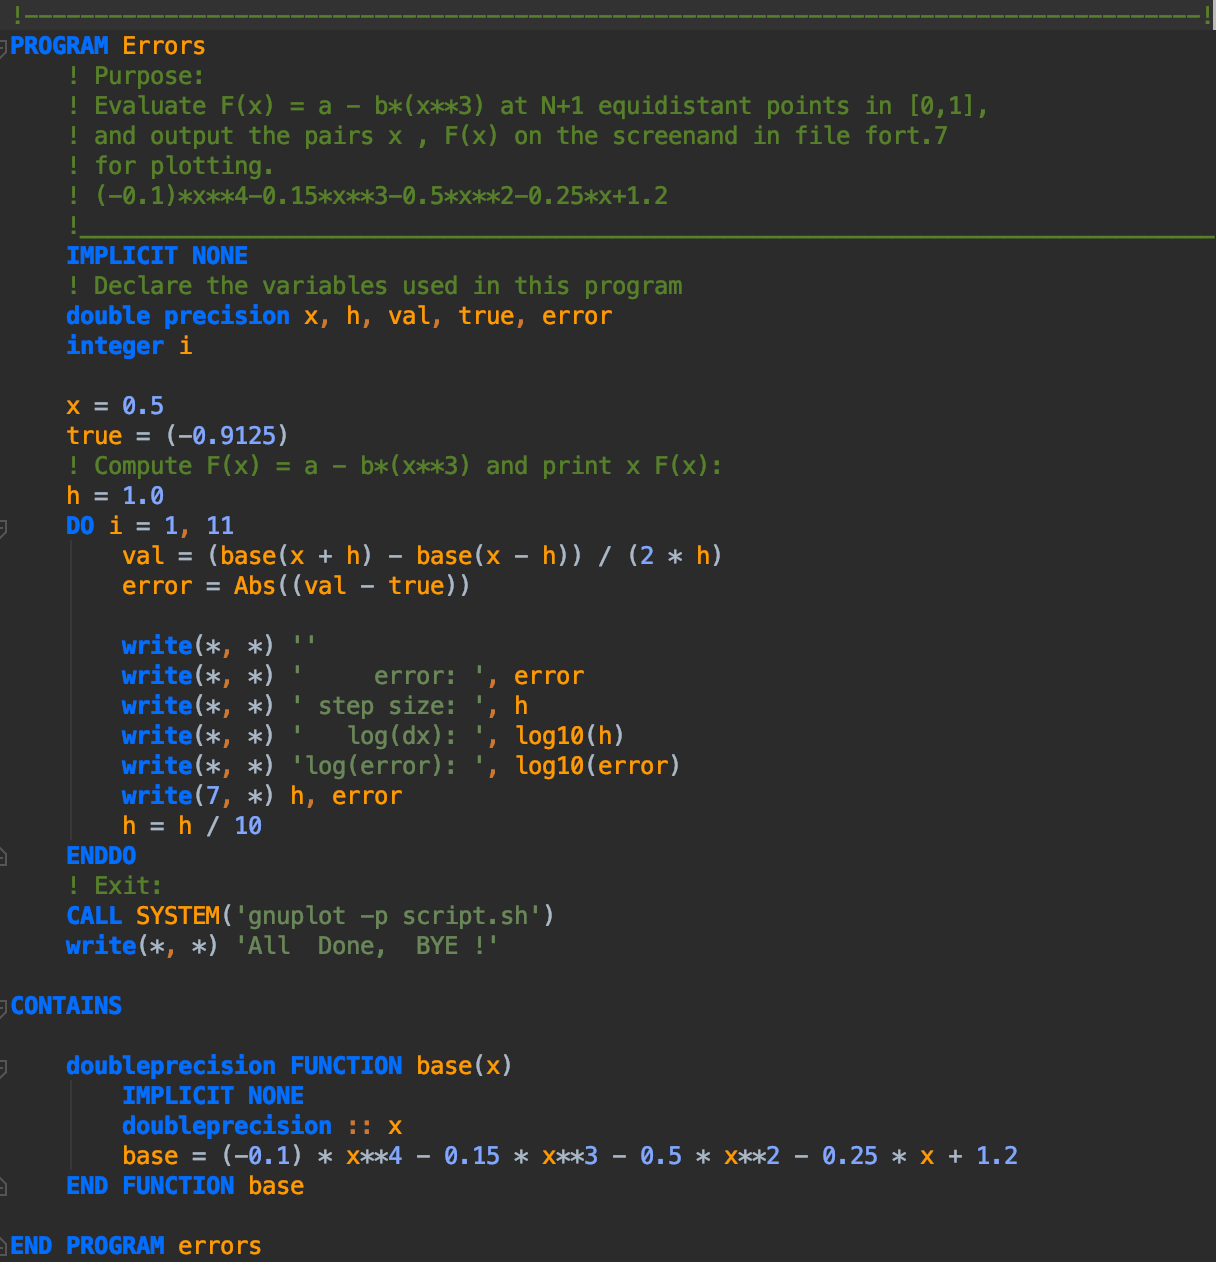
\includegraphics[width=.988975\linewidth]{FortranCode.png}
			%\caption{Fortran program code}
		\end{figure}
		
		\begin{figure}[h]
			\centering
			%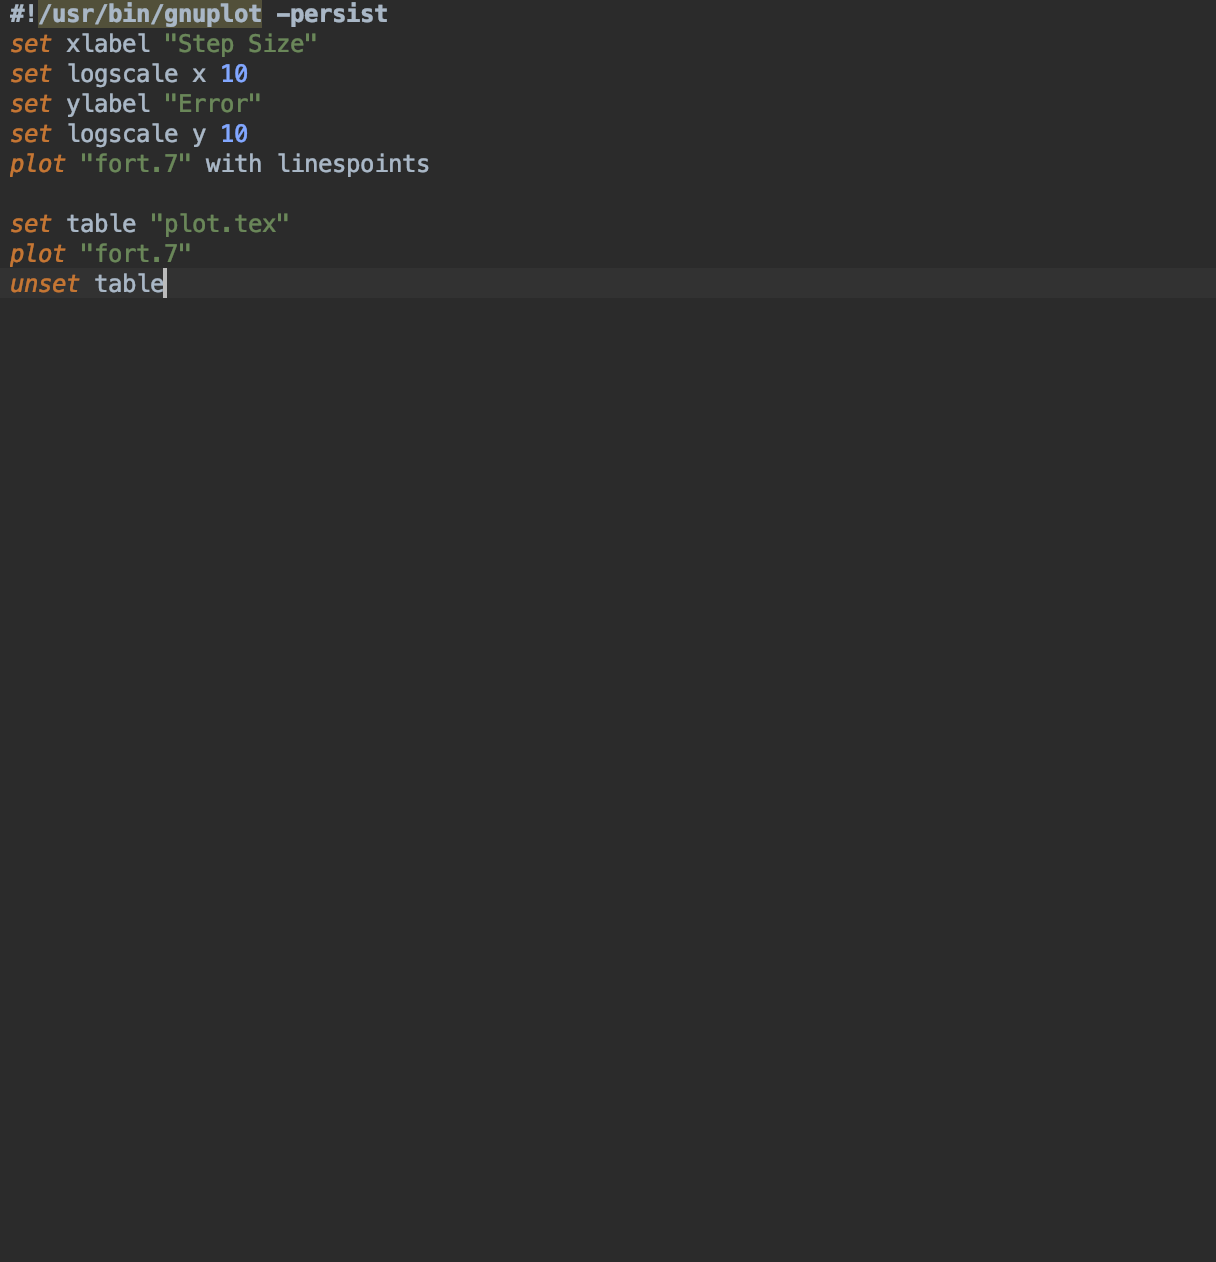
\includegraphics[width=\linewidth]{GnuplotCode.png}
			%\caption{Script for gnuplot to set up the graph correctly}
		\end{figure}


\end{document}
